\section{Fundamentals}
\label{sec:fundamentals}

\subsection{SEE}
The \gls{see} project aims to connect people regardless of space in a virtual room to analyze code structure. 
The Unity based project uses various types of code visualization (\cite{koschke}, \cite{DBLP:conf/iwsc/KoschkeS21}). 
One scenario uses the metaphor of cities to illustrate the code structure of an application.
An example of such an \gls{city} can be seen in figure \ref{fig:see_example}.
Such city graphs can be imported from \gls{glx} files.
Elements that represent building will be called \glspl{node} and underlying platform will be called \gls{plane}.

In the current state of the SEE project the virtual room can be accessed with VR glasses or a desktop computer.
This thesis aims to add an implementation of \gls{see} for \gls{android} devices.
This shall help developers to collaborate on software projects as freely as possible.
\begin{figure}[htb]
    \centering
    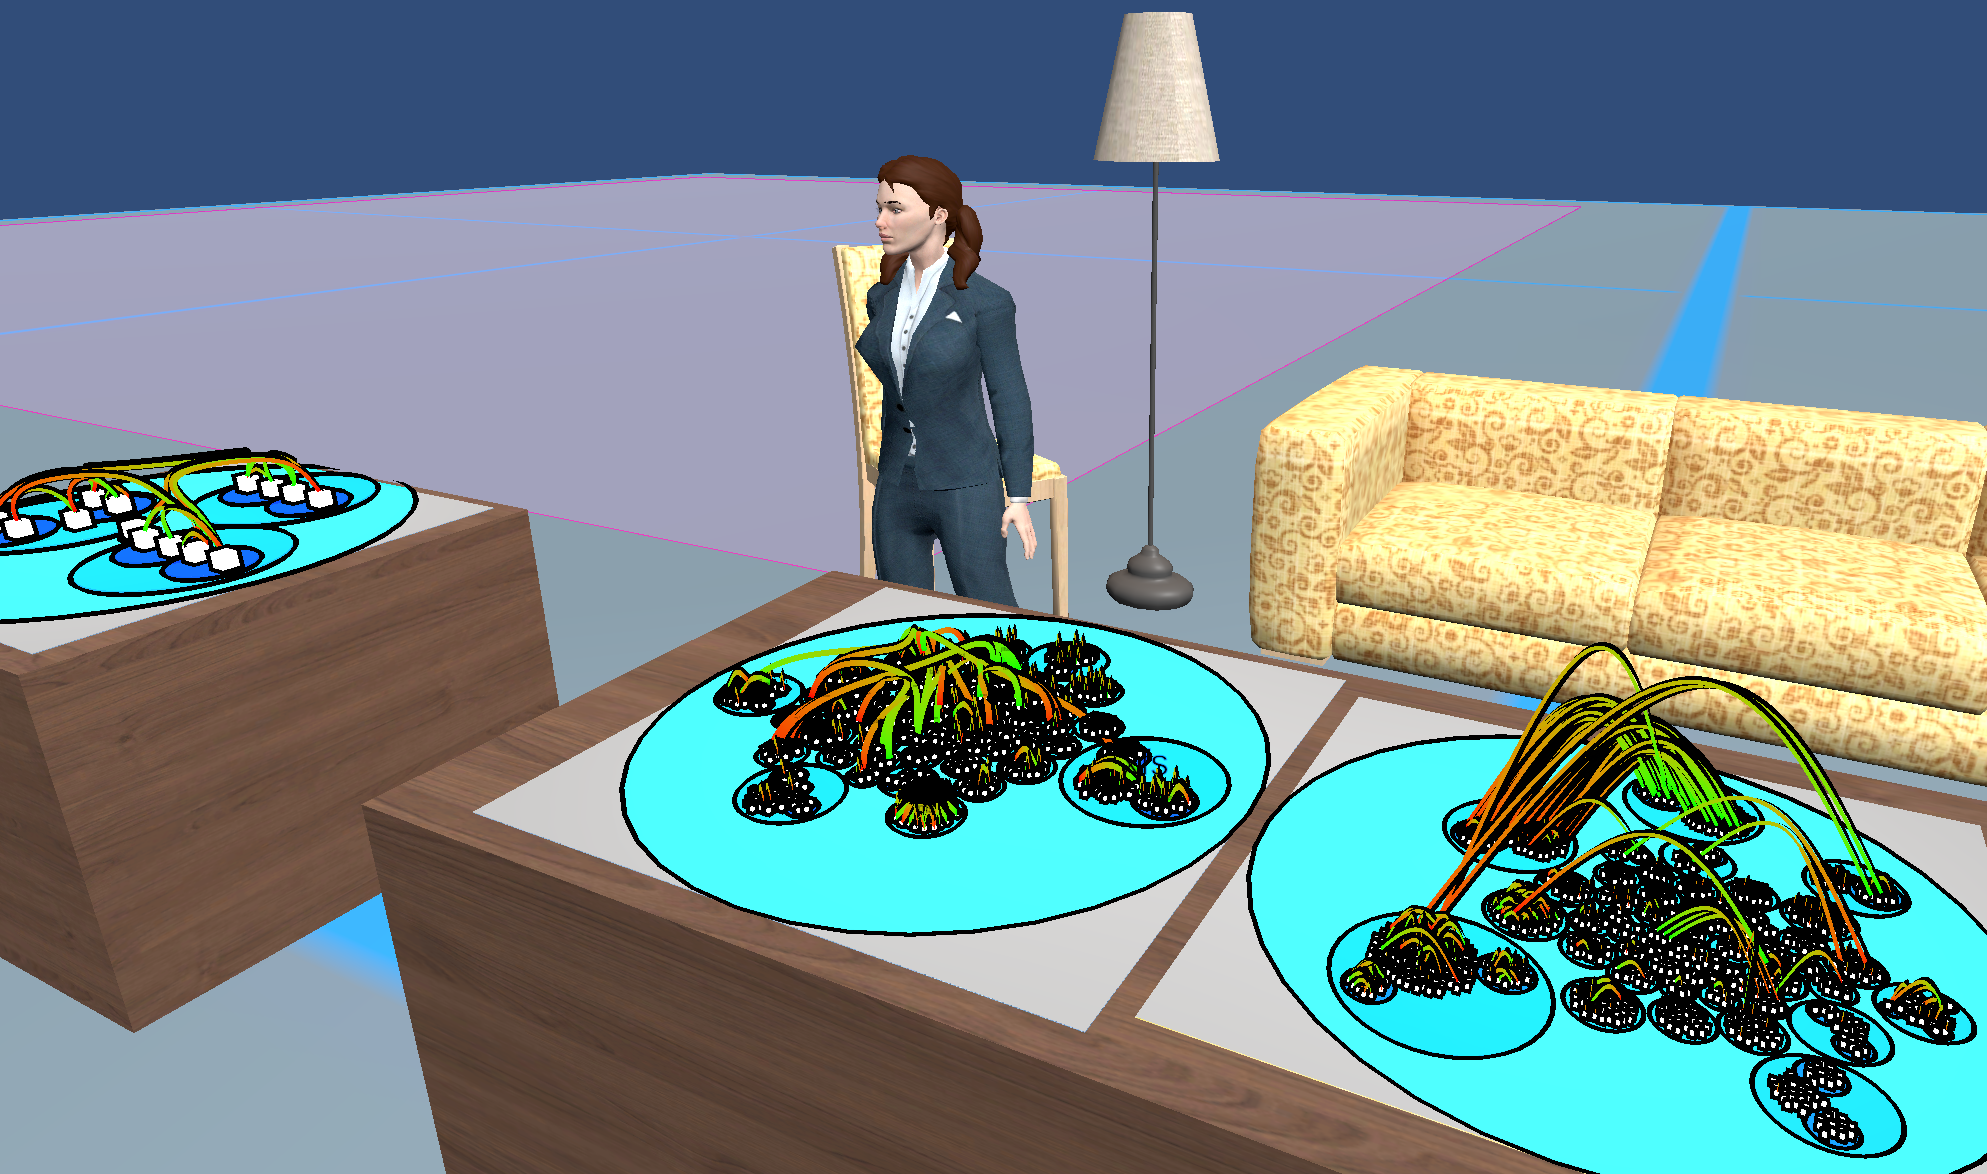
\includegraphics[width=1\textwidth]{Fundamentals/img/SEE.png}
    \caption{An example of \gls{see} used for the user study in chapter \ref{section:evaluation}}
    \label{fig:see_example}
\end{figure}
\subsection{Code Cities}
A \gls{city} is an approach of visualizing software projects.
An example of a \gls{city} by \cite{wettel2007visualizing} can be seen in figure \ref{fig:city_example}.
Since the representation is three-dimensional many metrics can be visualized in a single \gls{city}.
Code Cites could use, as an example, the metrics number of classes as building height, number of attributes as base size and the and the nesting level of a package as the building color (\cite{wettel2008visual}).
The \gls{city} provides an overview of the represented system and by walking around it in \gls{see} the user can get an idea of the structure of the represented system.
On challenge of representing large code bases is the overwhelming amount of information.
Therefore, using metaphors as the \gls{city} aims to avoid overwhelming the user with too much abstract information (\cite{Wettel2008}).
\begin{figure}[htb]
    \centering
    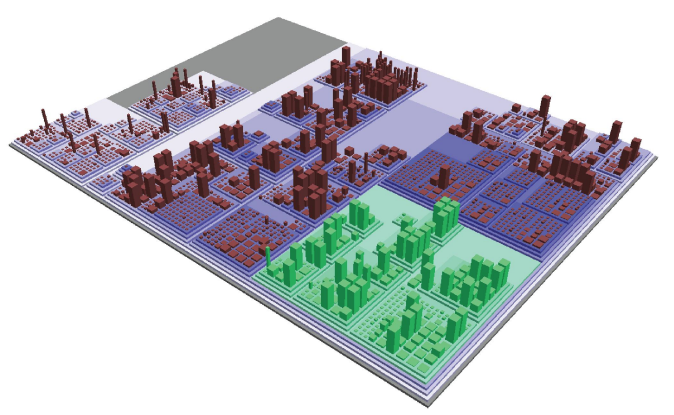
\includegraphics[width=1\textwidth]{Fundamentals/img/code_city.png}
    \caption{An example for a \gls{city} by \cite{wettel2007visualizing}}
    \label{fig:city_example}
\end{figure}

\subsection{Unity}
\gls{unity}\footnote{https://unity.com/ (last visited: 22.06.22, 2:39)} is a cross-platform game engine that has been released in June 2005.
The engine is not only popular for games but also for other industries regarding architecture, automotive or film.
Unity uses C\# as a programming language and is used 1.5 million active developers every month. 
\subsubsection{Ray Casting}
\label{sec:ray}
\subsubsection{Multi-Platform}
\subsubsection{Debugging and Testing}
Unity remote
\subsection{Android Interface Design}
